%
% schlange.tex
%
% (c) 2021 Prof Dr Andreas Müller, OST Ostschweizer Fachhochschule
%
\documentclass[tikz]{standalone}
\usepackage{times}
\usepackage{amsmath}
\usepackage{txfonts}
\usepackage[utf8]{inputenc}
\usepackage{graphics}
\usetikzlibrary{arrows,intersections,math,calc}
\usepackage{ifthen}
\begin{document}

\newboolean{showgrid}
\setboolean{showgrid}{false}
\def\breite{4}
\def\hoehe{4}
\def\a{47}
\def\r{3.3}
\def\skala{0.95}

\begin{tikzpicture}[>=latex,thick,scale=\skala]

\begin{scope}[xshift=-7.4cm,yshift=-1.2cm]
	\clip (-3.6,-2.2) rectangle (3.6,5.1);

	\fill[color=blue!20] (0,0)
		-- ({180-\a}:{0.4*\r}) arc ({180-\a}:180:{0.4*\r})
		-- cycle;
	\node[color=blue] at ({180-\a/2}:{0.3*\r}) {$\vartheta$};

	\fill[color=blue!20] (0,{\r/sin(\a)})
		-- ($(0,{\r/sin(\a)})+({270-\a}:{0.3*\r})$)
			arc ({270-\a}:270:{0.3*\r})
		-- cycle;
	\node[color=blue] at ($(0,{\r/sin(\a)})+({270-\a/2}:{0.2*\r})$)
		{$\vartheta$};


	\draw (0,0) circle[radius=\r];
	\draw[->] (0,-3.0) -- (0,5);
	\draw ({-\r-0.2},0) -- ({\r+0.2},0);
	\fill (0,0) circle[radius=0.06];

	\draw (0,0) -- ({180-\a}:\r);
	\node at ({180-\a+3}:{0.65*\r}) [above right] {$1$};

	\draw[color=red,line width=1.4pt]
		({180-\a}:\r) -- (0,{\r/cos(90-\a)});
	\fill[color=red] ({180-\a}:\r) circle[radius=0.08];
	\fill[color=red] (0,{\r/cos(90-\a)}) circle[radius=0.08];
	\node[color=red] at (-1.0,3.7) [left] {$r=\cot\vartheta$};
	\node[color=red] at ({180-\a}:\r) [above left] {$P$};
	\node[color=red] at (0,{\r/sin(\a)}) [right] {$Q$};
\end{scope}

% Povray Bild
\node at (0,0) {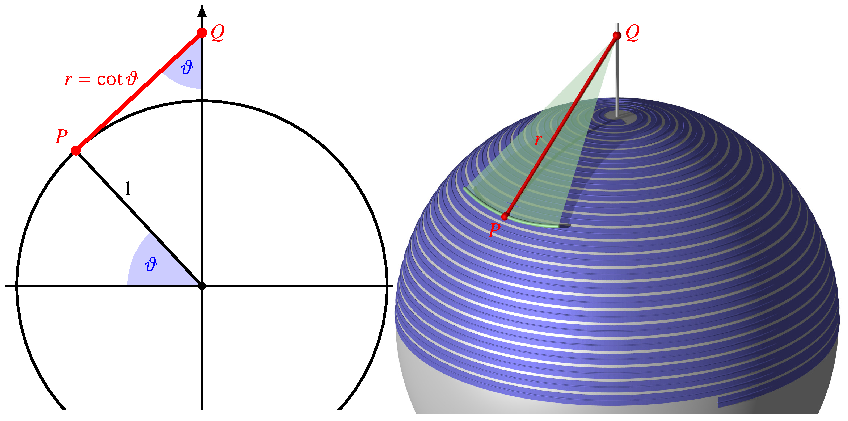
\includegraphics[width=7.6cm]{schale.jpg}};

% Gitter
\ifthenelse{\boolean{showgrid}}{
\draw[step=0.1,line width=0.1pt] (-\breite,-\hoehe) grid (\breite, \hoehe);
\draw[step=0.5,line width=0.4pt] (-\breite,-\hoehe) grid (\breite, \hoehe);
\draw                            (-\breite,-\hoehe) grid (\breite, \hoehe);
\fill (0,0) circle[radius=0.05];
}{}

\node[color=red] at (-1.4,1.4) {$r$};
\node[color=red] at (-2.2,-0.2) {$P$};
\node[color=red] at (0,3.3) [right] {$Q$};

\end{tikzpicture}

\end{document}

